% Number 326
% CVPMG Units
% Chase after time pause: problem-solving, assumption
% JG

% Watermark
\AddToShipoutPicture*{\BackgroundPic}

\addtocounter {ProbNum} {1}

%\begin{floatingfigure}[r]{.3\textwidth}
%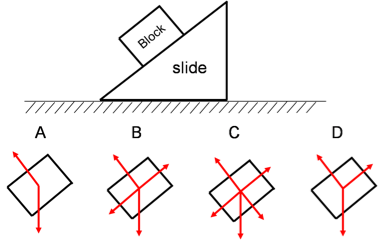
\includegraphics[scale=.4]{/Users/jgates/desktop/latex/pics/incline3.png}
%\end{floatingfigure}
 
{\bf \Large{\arabic{ProbNum}}}A real police car chases down a stolen sturgeon truck.  The police car is sitting by the side of the road when the truck flies by at ${35~\tfrac{m}{s}}$.  The police officer takes 1.5 seconds to react, but we'll assume that she can get the car up to speed instantly.

%\begin{center}
%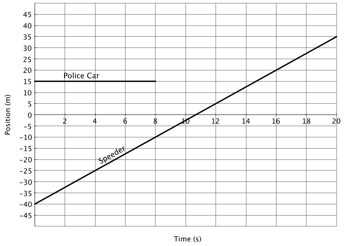
\includegraphics[scale=.87]{/Users/jgates/desktop/latex/pics/cvpm2.png}
%\end{center}

\bigskip
How fast will she have to go in order to catch the speeder within 2 km? Use graphical problem-solving.
 
\vfill
Graph (with a dotted line for the police car, but on the same axes as before) a more realistic scenario, where she requires time to get up to full speed.

\bigskip

What will this do to the top speed that will be required to catch the truck within 2 km?  Make sure that your graph agrees with this!
\vspace{15mm}
\newpage
